\documentclass[water,article,accept,pdftex,moreauthors]{Definitions/mdpi}
%\usepackage{showframe}
\usepackage{algorithm}
\usepackage{algorithmic}

% MDPI internal commands - do not modify
\firstpage{1}
\makeatletter
\setcounter{page}{\@firstpage}
\makeatother
\pubvolume{16}
\issuenum{14}
\articlenumber{1965}
\pubyear{2024}
\copyrightyear{2024}
\externaleditor{Academic Editor: }
\datereceived{7 June 2024}
\daterevised{4 July 2024} % Comment out if no revised date
\dateaccepted{9 July 2024}
\datepublished{11 July 2024}
%\datecorrected{} % For corrected papers: "Corrected: XXX" date in the original paper.
%\dateretracted{} % For corrected papers: "Retracted: XXX" date in the original paper.
\hreflink{https://doi.org/10.3390/w16141965} % If needed use \linebreak
%\doinum{}
%\pdfoutput=1 % Uncommented for upload to arXiv.org
%\CorrStatement{yes}  % For updates


% %% preamble
% Full title of the paper (Capitalized)
\Title{A Stream-Order Family and Order-Based Parallel River Network Routing Method}%Please note title change.

% MDPI internal command: Title for citation in the left column
\TitleCitation{A Stream-Order Family and Order-Based Parallel River Network Routing Method}

% Author Orchid ID: enter ID or remove command
\newcommand{\orcidauthorZ}{0000-0001-7580-9128}
\newcommand{\orcidauthorY}{0000-0002-5629-4795}

% Authors, for the paper (add full first names)
\Author{Xi Yang $^{1}$, Chong Wei $^{1}$, Zhiping Li $^{2}$, Heng Yang $^{3}$\orcidY{} and Hui Zheng $^{4,}$*\orcidZ{}}

% MDPI internal command: Authors, for metadata in PDF
\AuthorNames{Xi Yang, Chong Wei, Zhiping Li, Heng Yang, and Hui Zheng}

% MDPI internal command: Authors, for citation in the left column
\AuthorCitation{Yang, X.; Wei, C.; Li, Z.; Yang, H.; Zheng, H.}

% Affiliations / Addresses (Add [1] after \address if there is only one affiliation.)
\address{%
$^{1}$ \quad College of Surveying and Geo-Informatics, North China University of Water Resources and Electric Power, Zhengzhou 450046, China; yangxi940822@gmail.com (X.Y.); dixin313@163.com (C.W.)\\
$^{2}$ \quad College of Geosciences and Engineering, North China University of Water Resources and Electric Power, Zhengzhou 450045, China; lizhiping@ncwu.edu.cn \\
$^{3}$ \quad Science and Technology Research Institute, China Three Gorges Corporation, Beijing 100038, China; yang\_heng2@ctg.com.cn \\
$^{4}$ \quad Laboratory of Regional Climate-Environment Research for Temperate East Asia, Institute of Atmospheric Physics, Chinese Academy of Sciences, Beijing 100029, China }

% Contact information of the corresponding author
\corres{Correspondence: zhenghui@tea.ac.cn}

% Abstract (Do not insert blank lines, i.e. \\)
\abstract{River network routing's significance in reach-level flood forecasting over extensive domains is growing, requiring considerable computational resources for modeling networks comprising thousands to millions of reaches. Parallel computation plays a central role in timely forecasting in such cases. However, the sequentiality of upstream-to-downstream flow paths within river networks poses a significant challenge for parallelization. This study introduces a family of stream orders and an associated order-based parallel routing approach. We assign each reach an order that falls between one more than the maximum order of its upstream reaches and one less than the order of its downstream reach. This strategy enables the parallel simulation of reaches with identical orders while sequentially processing those with different orders, thus maintaining the crucial upstream-to-downstream dynamic. To further enhance parallel scalability, we strategically relax the upstream-to-downstream relationship along the longest flow paths, dividing the network into independent subnetworks and introducing halo reaches to mitigate the impact of inexact inflows. We validate our approach using China's Yangtze River basin, the country's largest river network with 53,600 fully connected reaches. Employing a conceptual parallel execution machine, we demonstrate that our method achieves 80\% parallel efficiency with up to 25 processors. By strategically introducing breakpoints, we further enhance scalability, enabling efficient simulations on 77 processors while maintaining 80\% efficiency. These results highlight the scalability and efficiency of our methods for large-scale, high-resolution river network modeling within Earth system models. Our study also lays a theoretical groundwork for optimizing stream orders and halo reach placements, crucial for advancing river network modeling.}

% Keywords
\keyword{stream order; river network routing; parallel computing; flood}

% %%
% document
\begin{document}

\section{Introduction}

River network routing has become increasingly essential for flood forecasting at the reach level over large domains, such as entire nations or even globally, as~demonstrated by various studies~\cite{alfieri2013HESS, david2016ESS, maidment2017JAWRA, lin2018JHM, read2023JAWRA}. The~National Water Model of the United States stands out as a successful example. It has been operational since 2016, providing flood forecasts for millions of reaches across the country. Its forecasts have effectively guided emergency responses during Hurricane Harvey~\cite{maidment2017JAWRA, read2023JAWRA}. The~Global Flood Awareness System is another significant example. Its forecasts cover the entire globe, including data-scarce regions. The~forecasts have demonstrated their value for targeted humanitarian disaster prevention actions in countries such as Uganda~\cite{alfieri2013HESS, coughlan_de_perez2016HESS}. More large-domain flood forecasting systems that leverage river network routing are actively being developed worldwide, including the recently established European-wide Flood Early Warning System~\cite{najafi2024NC, thober2019GMD}.

\textls[-5]{River network routing in flood forecasts is urgently focusing on shorter reaches~\cite{maidment2017JAWRA, coughlan_de_perez2016HESS, najafi2024NC, wada2016JAMES}}. The~use of shorter reaches and the accompanying frequent time-stepping is crucial for resolving fine-scale features and processes that significantly impact larger-scale river water flow patterns~\cite{yamazaki2009HESS, thober2019GMD, mizukami2021JAMES, nguyen-quang2018GMD}. This resolution of fine-scale water flow features within the river network enables local flood impact assessments to be highly relevant to individual people and infrastructures. These assessments are essential, providing targeted information instrumental for effective disaster prevention and response actions~\cite{maidment2017JAWRA, coughlan_de_perez2016HESS}.

Large-domain and fine-scale river network routing demands substantial computational resources~\cite{yamazaki2013WRR, liu2014EMS, mizukami2021JAMES, david2015WRR, liu2023JH}. Considering the constraints imposed by limited computational resources, flood forecasting systems must balance the need for detailed fine-scale modeling over broad domains with the necessity of timely forecasts. To~reconcile these competing demands, the~implementation of parallel processing in river network routing is essential. Parallel processing is crucial for enhancing computational efficiency and directly contributes to meeting the timeliness requirements of flood~forecasts.

However, the~parallelization of river network routing presents considerable challenges, primarily due to the inherent sequentiality of the river flow from upstream to downstream within the networks. The~flow in any given reach is dependent on the flow conditions in its upstream reaches. It is imperative that a parallel routing algorithm respects this upstream-to-downstream dependency. When this dependency is a constraint, the~parallel routing needs to revert to a sequential approach from upstream to downstream. Additionally, the~spatial variability within river networks, marked by differences in channel widths, slopes, and~flow velocities, adds to the complexity of parallelization. This variability necessitates dynamic load-balancing techniques to prevent computational resources from being underutilized or overburdened. Consequently, it is critical to develop robust parallel algorithms that can accommodate the diverse dynamics and inherent sequentiality within river networks effectively, ensuring that simulation results are physically plausible and accurate~\cite{david2013WRR, mizukami2021JAMES, liu2014EMS, liu2023JH}.

Several parallelization methods exist, such as domain decomposition~\cite{mizukami2021JAMES, liu2023JH} and halo reaches~\cite{david2013WRR}. Domain decomposition involves partitioning river networks into independent tributaries and interconnected mainstreams. The~tributaries are then allocated to various processors for concurrent simulation, while the mainstreams are processed in an upstream-to-downstream sequence. However, the~parallelization scalability is limited. As~the number of processors increases, the~distribution of reaches within the tributaries diminishes, and~the mainstream reaches become more dominant~\cite{mizukami2021JAMES}. In~an extreme scenario with an infinite number of processors, the~majority of river reaches would be classified as mainstreams, effectively rendering the routing process predominantly~sequential.

With the halo-reach method, the~river network is divided into independent subnetworks, each of which is simulated in parallel without maintaining an upstream-to-downstream relationship at their boundaries~\cite{david2015WRR}. To~mitigate the inaccuracies arising from this artificial division, halo reaches are prepended upstream of each subnetwork. These halo reaches serve to buffer the impact of boundary inaccuracies. This strategy offers scalability and efficiency, although~careful configuration of the halo reaches is essential to ensure simulation accuracy~\cite{david2013WRR}.

In this paper, we introduce a stream-ordering method and an order-based parallel routing approach to address the challenges of parallel river network routing. Our method sets itself apart from the halo-reach method through its strict adherence to the upstream-to-downstream sequence, ensuring that simulations are both physically plausible and accurate. Incorporating parallel scalability as a core design principle, our method is exceptionally efficient. In~an ideal scenario with unlimited processors, the~computation time of our method would closely match that of sequential routing along the river's longest path, significantly outperforming the domain-decomposition method previously~discussed.

The structure of this paper is as follows. Section~\ref{sec:methods} details our proposed stream-ordering and order-based parallel routing methods. These methods are tested in the Yangtze River basin, the~largest river basin in China. Section~\ref{sec:domain} describes the study area and the river network geometry dataset used. Section~\ref{sec:results} presents an analysis of the parallel scalability and efficiency of our method. Finally, Section~\ref{sec:conclusions} summarizes our~findings.

\section{Stream Orders and Parallel River Network~Routing}
\label{sec:methods}

Our parallel river network routing method encompasses two key components. The~first is the stream-ordering method, which systematically assigns an order to each reach within the network based on its connectivity and flow direction. The~second is the order-based parallel routing approach, which enables parallel simulation of reaches that share the same order while reverting to sequential processing for those of different orders. Section~\ref{sec:stream_order} introduces the stream-ordering method, Section~\ref{sec:comparison} briefly compares the proposed method with existing methods, and~Section~\ref{sec:parallel_machine} details the order-based parallel routing~approach.

\subsection{A Family of Stream Orders Designed for Parallel River~Routing}
\label{sec:stream_order}

Table~\ref{tab:zheng_order} describes the proposed stream-ordering method, and~Figure~\ref{fig:zheng_order} illustrates the method using a simple synthetic river network. The~method consists of two rules: (1) a reach's order falls within an integer range that is one more than the highest order of its upstream reaches and one less than the order of its downstream reach, and~(2) the order value is an integer ranging from one up to the number of the reaches along the longest flow path within all the river networks under examination. This ordering ensures that reaches with identical orders are free from upstream-downstream dependencies, allowing for parallel~processing.


\begin{table}[H]
    \caption{The proposed methods of stream ordering and the upper and lower limits of the feasible stream-order values. The~Strahler and Shreve orders are included for~comparison.\label{tab:zheng_order}}

    \begin{adjustwidth}{-\extralength}{0cm}

        \newcolumntype{C}{>{\centering\arraybackslash}m{42em}}
        \newcolumntype{c}{>{\centering\arraybackslash}m{13em}}
        \begin{tabularx}{\fulllength}{c C}
            \toprule
            \textbf{Ordering Method}                         & \textbf{Rules of Ordering}
            \\
            \midrule

            The proposed stream-ordering method              & \begin{enumerate}
                                                                   \item A reach's order ranges from the maximum of its upstream orders plus one to one less than the minimum of its downstream orders.
                                                                   \item The order value is an integer ranging from one up to the number of reaches along the longest flow path within all the river networks under examination. In~other words, the~order of the uppermost reaches is at least one, while the order of the outlet reaches is at most the total number of reaches along the longest flow path.
                                                                         \vspace{-6pt}              \end{enumerate}
            \\
            Lower limit of the feasible stream-order values,
            as illustrated in Figure~\ref{fig:zheng_order}a. & \begin{enumerate}
                                                                   \item The uppermost reaches are assigned an order of one.
                                                                   \item The order of the remaining reaches in the networks is one plus the highest order of their upstream reaches.
                                                                         \vspace{-6pt}   \end{enumerate}
            \\
            Upper limit of the feasible stream-order values,
            as illustrated in Figure~\ref{fig:zheng_order}b. & \begin{enumerate}
                                                                   \item Outlet reaches are assigned an order equivalent to the number of reaches along the longest flow path.
                                                                   \item The order of the remaining reaches is one less than the order of their downstream reach.
                                                                         \vspace{-6pt}         \end{enumerate}
            \\
            The Strahler stream-ordering method,
            as illustrated in Figure~\ref{fig:zheng_order}d. & \begin{enumerate}
                                                                   \item The uppermost reaches are assigned an order of one.
                                                                   \item If two or more upstreams have the highest order, the~reach's order is one more than that order.
                                                                   \item Otherwise, the~reach's order is the highest order of its upstreams.
                                                                         \vspace{-6pt}           \end{enumerate}
            \\
            The Shreve stream-ordering method,
            as illustrated in Figure~\ref{fig:zheng_order}e. & \begin{enumerate}
                                                                   \item The uppermost reaches are assigned an order of one.
                                                                   \item If a reach has a single upstream, its order is one plus the upstream's order~\textsuperscript{1}.
                                                                   \item Otherwise, the~reach's order is the arithmetic sum of the orders of its upstreams.
                                                                         \vspace{-6pt}         \end{enumerate}
            \\
            \bottomrule
        \end{tabularx}
    \end{adjustwidth}
    \noindent{\footnotesize{\textsuperscript{1} We added this rule to the commonly used Shreve ordering method. This addition is essential to ensure that parallel routing maintains the correct upstream-to-downstream sequence.}}

\end{table}
\vspace{-6pt}

\begin{figure}[H]
    \begin{center}
        \includegraphics[width=4cm]{fig/stream_order.pdf}
        \hspace{0.5cm}
        \includegraphics[width=4cm]{fig/stream_order_r.pdf}
        \hspace{0.5cm}
        \includegraphics[width=4cm]{fig/stream_order_a.pdf}

        \includegraphics[width=4cm]{fig/stream_order_strahler.pdf}
        \hspace{0.5cm}
        \includegraphics[width=4cm]{fig/stream_order_shreve.pdf}
    \end{center}
    \caption{Illustration of and comparison between different stream-ordering methods. (\textbf{a}) Lower limits of the feasible stream-order values from our proposed methods. (\textbf{b}) The upper limits of the feasible stream-order values from our proposed methods. (\textbf{c}) Another feasible set of stream-order values conforming to the two rules of our proposed ordering methods, as described in Table~\ref{tab:zheng_order}. (\textbf{d}) The Strahler stream-ordering method. (\textbf{e}) The Shreve stream-ordering~method. \label{fig:zheng_order}}
\end{figure}


The two ordering rules allow for a spectrum of feasible stream-order values. The~lower and upper bounds of the feasible values for each reach can be estimated as follows, as~described in Table~\ref{tab:zheng_order} and illustrated in Figure~\ref{fig:zheng_order}a,b. The~lower bounds are calculated by repeating the following two steps: (1) assigning the upmost reaches an order of one, and~(2) setting a reach's order to one plus the highest upstream order. Conversely, the~upper bounds are determined by (1) designating the outlet reach an order equivalent to the number of reaches along the longest flow path, and~(2) subtracting one from the downstream reach's~order.


\subsection{Comparison with Existing Stream-Ordering~Methods}
\label{sec:comparison}

Our method of stream ordering is inspired by several foundational studies. The~mizuRoute river network routing model, for~instance, employs the Strahler stream order to segment mainstreams into branches~\cite{mizukami2021JAMES}. Within~each branch, reaches are sequentially simulated from upstream to downstream, while branches of the same Strahler order are processed in parallel. This approach underscores the potential of order-based parallelism. However, the~Strahler ordering method, as~depicted in Figure~\ref{fig:zheng_order}d, categorizes branches rather than individual reaches, leading to a granularity too coarse for efficient parallel routing. The~disparity in the number of branches across Strahler orders and in the number of reaches in a branch introduces significant variability in the computational load, posing a considerable challenge for load balancing and scalable parallel~processing.

Recognizing these challenges, a~method that assigns stream orders directly to river reaches could enable more granular parallelization. The~Shreve stream-ordering method falls into this category. However, the~method is too finely grained. The~excessive granularity in the context of parallel routing can be demonstrated through the following theoretical reasoning: In an ideal scenario with unlimited processors, the~computation time for parallel routing would be equivalent to that of computing the reaches sequentially along the longest flow path. For~instance, as~shown in Figure~\ref{fig:zheng_order}e, there are five reaches along the longest flow path. An~ideal ordering method would assign five unique order values, and~the computation time would be five times the time required to compute a single reach. However, the~Shreve method assigns six unique order values. If~the number of processors is unlimited, the~computation time would be six times the time taken to compute a single reach. This excessive granularity of Shreve ordering leads to a suboptimal degree of~parallelization.

\textls[-10]{The Spatially Explicit Integrated Modeling System (SEIMS) model introduces a novel layer-based parallelism~\cite{liu2014EMS, liu2016EMS, zhu2019EMS}, which is considered to have an ideal granularity. The~model} stratifies reaches by their topological distance from the outlet. Reaches within the same layer are processed in parallel, with~the layers being sequenced. Yet, the~allocation of a reach to a specific layer is predetermined by the river network's topography. If~the number of reaches in a layer does not match the number of processors, processor idleness ensues~\cite{liu2014EMS, zhu2019EMS}. However, the~SEIMS model lacks the flexibility required to optimize reach distribution across~layers.

Our proposed ordering method offers a more adaptable alternative to the SEIMS model. On~one hand, the~lower~(Figure~\ref{fig:zheng_order}a) and upper~(Figure~\ref{fig:zheng_order}b) bounds of our proposed orders parallel the SEIMS layers assigned using an upstream-downstream strategy~\cite[Figure 6b]{zhu2019EMS} and a downstream-upstream strategy~\cite[Figure 6c]{zhu2019EMS}, respectively. Additionally, our proposed ordering method allows for variations in the stream-order values between the lower and upper bounds, provided that the two rules are satisfied. This flexibility enables the optimization of the reach distribution, potentially minimizing processor idleness and enhancing parallel efficiency, as~evidenced in Section~\ref{sec:optimization_yangtze}.

Our proposed ordering method can also incorporate the halo-reach method to further enhance parallel scalability. If~the number of processors allocated for parallel river network routing is sufficiently large, the~computation time will predominantly be dictated by the reaches along the longest flow path. By~strategically inserting halo reaches upstream of select reaches along the longest flow path, the~river network can be effectively partitioned into subnetworks with shorter longest flow paths. This partitioning will enable the application of our proposed ordering methods to each subnetwork, thereby enhancing parallel scalability. In~comparison with the existing halo-reach method, the~use of halo reaches with our proposed ordering method should be judicious, reserved for scenarios where the longest flow path emerges as the primary determinant of computation time. This~judicious use will minimize the impact of inexact inflows on the artificially partitioned subnetworks, ensuring simulation~accuracy.

\subsection{A Conceptual Shared-Memory Parallel Execution Machine for River Network~Routing}
\label{sec:parallel_machine}

In this study, we utilize a conceptual shared-memory parallel execution model to assess the parallel performance and scalability of our proposed stream-ordering method. This model offers a theoretical framework for evaluation, factoring out the impact of inefficient code implementation and hardware architectural differences. The~parallel performance and scalability metrics obtained are instrumental in guiding the optimization of the proposed stream~orders.

The conceptual machine is equipped with $m$ processors capable of simultaneously processing up to $m$ reaches. The~river networks under consideration comprise a total of $n$ reaches. The~machine selects groups of reaches from the river networks, beginning with the lowest order. Each group consists of reaches of the same order, which are selected randomly. The~size of each group does not exceed $m$. This process is repeated until all reaches have been simulated, as~outlined in Algorithm~\ref{alg:shared_memory}.

We disregard the time spent on fetching and potential data-saving operations. The~total computation time is quantified by the total number of groups required to process the entire river network. Parallel performance is gauged using the metrics of parallel speedup and efficiency. Parallel speedup is calculated as the ratio of the computation time for sequential simulation (i.e., the~total number of river reaches) to that for parallel simulation. Perfect scaling is achieved if the speedup ratio increases linearly with the number of processors. Parallel efficiency is determined by the ratio of the actual parallel speedup to the ideal speedup under perfect scaling conditions. This efficiency metric is crucial for evaluating the parallel performance and scalability of the proposed stream~orders.

During computation, there may be instances of processor idleness. This idleness is attributed to the mismatch between the number of reaches in a group and the number of available processors. Such idleness can diminish parallel efficiency and scalability. To~identify potential sources of this idleness, we calculate the computation deficiency for each individual reach. The~computation deficiency of a reach is defined as the ratio of the number of idle processors during the routing of the reach to the number of total processors. If~no processors are idle during the routing of a reach, the~computation deficiency is zero. If~idle processors are present, the~computation deficiency is positive; as the number of idle processors increases, the~deficiency approaches one. This metric is valuable for identifying reaches that contribute to processor idleness and for guiding the optimization of stream~orders.

\begin{algorithm}
    \caption{A shared-memory parallel execution machine for river network~routing.}
    \label{alg:shared_memory}
    \begin{algorithmic}
        \REQUIRE There are $n$ streams. $O_i \in \mathbb{Z}^{+}$ is the order of the $i$-th stream, $i = 1\cdots{}n$. The~order is sorted: $O_{i+1} - O_i \ge 0$.
        \REQUIRE The machine has $m$ processors. $m \in \mathbb{Z}^{+}$.
        \ENSURE The simulation of a stream must be after its upstream.
        \STATE $i \gets 1$ \COMMENT{the first stream of a group}
        \STATE $j \gets 1$ \COMMENT{the last stream of a group}
        \WHILE{$i \le n$}
        \FOR {$k = 1$ \TO $m$}
        \IF {$i + k - 1 \le n$ \AND $O_{i + k - 1} = O_i$}
        \STATE $j \gets i + k - 1$
        \ENDIF
        \ENDFOR
        \STATE \textbf{Parallel Simulation} Simulate the streams from $i$ to $j$ in parallel.
        \STATE $i \gets j + 1$
        \ENDWHILE
    \end{algorithmic}
\end{algorithm}

\vspace{-12pt}
\section{Experimental~Design}
\label{sec:domain}

We applied the proposed stream-ordering and order-based parallel routing methods to the Yangtze River, the~largest river network in China. The~river network is characterized by full connectivity among its reaches. This case provides a rigorous evaluation of our proposed methods at a substantial scale and under challenging conditions for parallel~routing.

For the delineation of the Yangtze River network, we employed the Multi-Error-Removed Improved-Terrain Hydrography (MERIT-Hydro) dataset~\cite{yamazaki2017GRL, yamazaki2019WRR}, a~global hydrography dataset with a 3 arc-second spatial resolution. This dataset includes a hydrologically adjusted digital elevation model, an~eight-direction flow model, flow accumulation area, river channel width, and~height above the nearest drainage. Our delineation process utilized the flow accumulation area and the eight-direction flow model. The~threshold for the flow accumulation area was set at 20 km\textsuperscript{2} for catchment delineation and 10 km\textsuperscript{2} for river centerline extraction. The~extraction yielded a single river network comprising 53,600 reaches (tributaries), which are shown in Figure~\ref{fig:domain}. We utilized the connectivity of the extracted river centerlines for subsequent analyses and employed the river geometry for graphical illustrations. The data can be found in the Supplementary~Materials.

Figure~\ref{fig:workflow} shows the workflow of this study. Initially, in~Section~\ref{sec:stream_order_yangtze}, we assign the Strahler, Shreve, and~the upper and lower bounds of our proposed stream orders to the Yangtze River network, adhering to the rules detailed in Table~\ref{tab:zheng_order} and depicted in Figure~\ref{fig:zheng_order}. Subsequently, in~Section~\ref{sec:parallelization_yangtze}, we assess the computational performance of the Shreve order and the proposed stream orders' upper and lower bounds using the conceptual shared-memory parallel execution machine described in Section~\ref{sec:parallel_machine}. We measure this performance in terms of parallel speedup and efficiency and evaluate its scalability with an increasing number of processors. We also pinpoint hotspots of computational deficiencies. Lastly, in~Sections~\ref{sec:optimization_yangtze} and \ref{sec:breakdown_yangtze}, we demonstrate that our proposed stream-ordering method can be optimized, guided by the measured computation deficiencies, and~can incorporate halo reaches into the longest flow path. This incorporation can significantly enhance computational performance and parallel~scalability.

\begin{figure}[H]
    \includegraphics[width=13.5 cm]{fig/domain.pdf}
    \caption{Yangtze River basin network delineated from the MERIT-Hydro dataset. The~black lines outline the national boundaries or coastal lines of China, providing a geographical context. The~color-coded lines depict the river reaches. Each color indicates the total number of reaches, encompassing the current reach and all upstream~reaches. \label{fig:domain}}
\end{figure}
\vspace{-9pt}
\begin{figure}[H]
    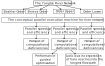
\includegraphics[width=11 cm]{fig/workflow.pdf}
    \caption{Diagram of~workflow. \label{fig:workflow}}
\end{figure}
\unskip

\section{Results and~Discussion}
\label{sec:results}
\unskip

\subsection{Stream Orders for the Yangtze River~Network}
\label{sec:stream_order_yangtze}

Figure~\ref{fig:spatial_distribution_yangtze} illustrates the spatial distribution of the proposed stream orders in the Yangtze River basin, juxtaposed with those of the Strahler and Shreve stream orders. The~Strahler system exhibits a narrow range of order values, with~a maximum value of eight observed in this case. This limited range restricts its application to parallelizing branches, akin to the mizuRoute model~\cite{mizukami2021JAMES}, rather than individual reaches. The~coarse granularity of the Strahler order poses challenges for achieving effective load~balancing.

In contrast, both the Shreve order and our proposed stream order offer sufficient granularity for order-based parallel routing. It is important to note that the Shreve order is applicable for parallel routing only when no upstream-downstream pairs share the same order value, a~condition that is coincidentally met in this study. However, the~Shreve order spans a range from 1 to 26,828, which is excessively broad. As~depicted in Figure~\ref{fig:cumulative_count_yangtze}, \mbox{2378 unique} Shreve order values are assigned to only one reach. This indicates an excessive granularity that undermines the scalability of the parallel routing. No matter how many processors are allocated, only one can work at a time while the others remain idle, waiting for the routing on the reach to be completed. This extensive range, coupled with the scarcity of reaches sharing the same order value, can lead to inefficiencies in~parallelization.

\begin{figure}[H]
    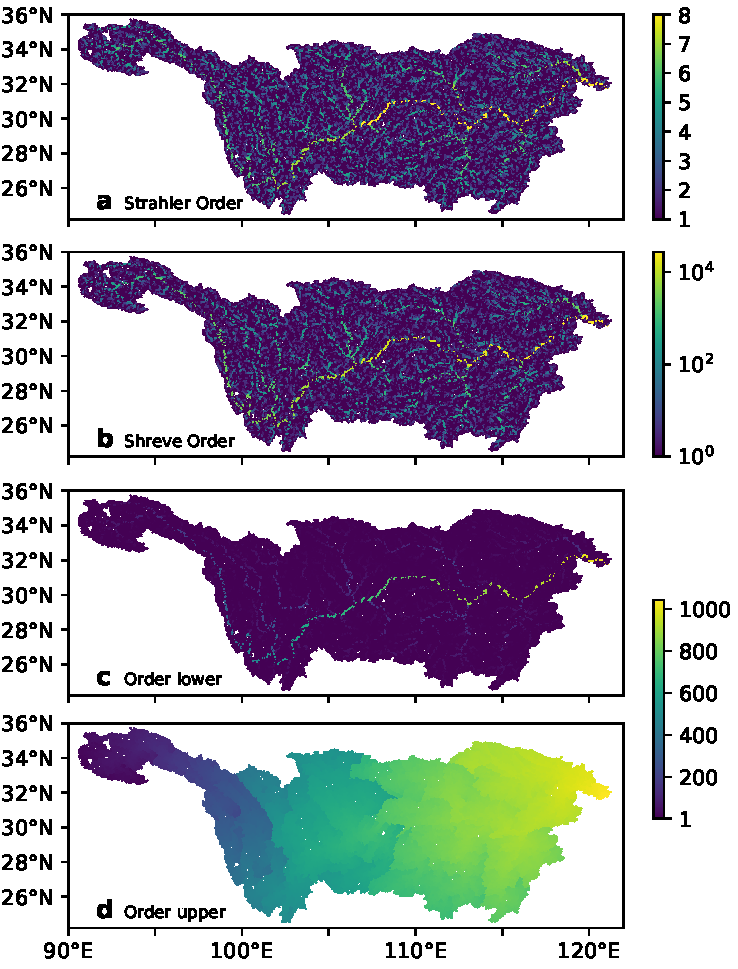
\includegraphics[width=13 cm]{fig/spatial_distribution_yangtze.pdf}
    \caption{Spatial distribution of stream orders over the Yangtze River basin. (\textbf{a}) The Strahler order. (\textbf{b}) The Shreve order. (\textbf{c}) The lower bounds of the proposed order family. (\textbf{d}) The upper bounds of the proposed order~family. \label{fig:spatial_distribution_yangtze}}
\end{figure}


Figure~\ref{fig:spatial_distribution_yangtze}c,d display the spatial distribution of the lower and upper bounds of our proposed order family, respectively. These bounds range from 1 to 1042, which corresponds to the number of reaches along the longest flow path. The~upper bound demonstrates an even distribution of order values throughout the river network, while the lower bound shows a greater concentration in the lower order values. For~the upper bound, a~limited number of order values are assigned to a small set of reaches, as~shown in Figure~\ref{fig:cumulative_count_yangtze}. The~balanced distribution of order values, along with the adequate granularity and the presence of sufficient reaches sharing the same order value, render the upper bounds of our proposed stream-order family particularly well suited for parallel river network~routing.


\begin{figure}[H]
    \includegraphics[width=13.5 cm]{fig/stream_count_yangtze.pdf}
    \caption{The count of stream-order values with a limited number of reaches. For~the sake of clarity, only stream orders with 16 or fewer reaches are~illustrated. \label{fig:cumulative_count_yangtze}}
\end{figure}
\unskip

\subsection{Parallelization Performance, Scalability, and~Hotspots of Computation~Deficiencies}
\label{sec:parallelization_yangtze}

Figure~\ref{fig:scalability_yangtze} displays the parallel speedup, efficiency, and~scalability of the proposed stream orders compared to the Shreve order. Initially, as~the number of processors increases, the~ideal speedup is linearly proportional to the number of processors allocated. When the allocated processors become abundant enough, the~parallelization process encounters a bottleneck due to the sequentiality along the longest flow path. The~black dashed lines in the figure indicate this theoretical limit. In~this instance, the~number of processors at which the ideal speedup reaches the theoretical limit is 51, which corresponds to the ratio of the total number of reaches in the river network to the number of reaches along the longest flow~path.

\vspace{-6pt}
\begin{figure}[H]
    \includegraphics[width=13.5cm]{fig/speedup_yangtze.pdf}
    \caption{Parallelization speedup (\textbf{a}) and efficiency (\textbf{b}) for the Shreve orders and the proposed stream orders, respectively. The~solid black lines represent the ideal speedup or efficiency under conditions of perfect scaling. The~dashed black lines indicate the limits imposed by the upstream-to-downstream sequentiality along the longest flow~path. \label{fig:scalability_yangtze}}
\end{figure}

The Shreve order shows the lowest parallelization performance and scalability. Its efficiency falls below 80\% as soon as the processor count exceeds six. When the number of processors is approximately 150 or above, the~speedup is nearly saturated. The~saturated speedup is significantly lower than the theoretical limit, with~a value of approximately 24.5. This value is close to the ratio of the total number of reaches to the number of unique Shreve order values (i.e., 24.87). This indicates that the low saturated speedup is likely due to the broad range of Shreve order values and the scarcity of reaches sharing the same order value, as~shown in Figures~\ref{fig:spatial_distribution_yangtze}~and~\ref{fig:cumulative_count_yangtze}.

The lower bounds of our proposed stream-order family offer superior speedup and efficiency compared to the Shreve order. As~the processor count increases, the~parallel speedup increases more rapidly. Once the number of processors exceeds approximately 280, further increases have minimal impact on speedup. The~saturation speedup closely matches the theoretical limit, indicating that the granularity of our proposed stream-order family is well suited for parallel processing. The~lower bounds also scale better. The~efficiency remains above 80\% when the number of processors is less than~14.

The lower bounds of the proposed stream-order family demonstrate better speedup and efficiency than the Shreve order. As~the allocated processor count escalates, the~parallel speedup increases at a more rapid rate than that of the Shreve order. However, once the number of processors surpasses about 280, the~enhancement in parallel speedup becomes negligible. The~saturation speedup is close to the theoretical limit, showing that the number of unique order values is appropriate. This suggests that our proposed stream-order family is ideally granular for parallel river network routing. Additionally, the~lower bounds showcase enhanced scalability, maintaining efficiency above 80\% when the processor count does not exceed~14.

The upper bounds demonstrate the best performance and scalability among the three methods. Efficiency is maintained above 80\% when the number of processors is 25 or fewer. As~the number of processors increases, the~speedup rapidly saturates, closely approaching the theoretical limits at a processor count of 141. These results indicate that the upper bounds of the proposed order family are particularly well suited for parallel river network routing. The~scalability of the upper bounds is either comparable to or surpasses those found in the existing literature~\cite{mizukami2021JAMES, liu2023JH}. It is important to note that scalability in this study is measured using a conceptual parallel execution model rather than with a real-world~implementation.


Figures~\ref{fig:computation_deficiency_yangtze}~and~\ref{fig:computation_deficiency_hist_yangtze}, respectively, illustrate the spatial distribution and the histogram of computation deficiencies within the Yangtze River network. These deficiencies were measured using 51 processors, the~point at which the ideal speedup aligns with the theoretical limit. For~the Shreve order and the lower bounds of the proposed stream-order family, reaches with significant computation deficiencies are primarily located in the mainstreams. This inefficiency arises from the limited number of mainstream reaches that share the same order values. In~contrast, due to the coarse granularity of the upper bounds, the~likelihood of computation deficiencies occurring is lower, and~they are more~concentrated.

The upper bounds exhibit a markedly different pattern, with~reaches showing high computation deficiencies predominantly found in the upstream reaches, especially in the headwater regions. The~greater number of upstream reaches compared to mainstream reaches makes it more probable that they will share order values. This sharing reduces the probability of processor idleness and computation deficiencies. The~contrasting patterns observed between the lower and upper bounds suggest that there is considerable potential for optimizing the order values to improve parallel~efficiency.

\begin{figure}[H]
    \includegraphics[width=11.5cm]{fig/computation_deficiency_yangtze.pdf}
    \caption{Computation deficiencies observed for routing each individual reach at a processor count of 51 for the Yangtze River~network. \label{fig:computation_deficiency_yangtze}}
\end{figure}
\unskip

\begin{figure}[H]
    \includegraphics[width=13.5cm]{fig/computation_cost_hist_yangtze.pdf}
    \caption{Histogram of computation deficiencies observed for the Yangtze River network at a processor count of~51. \label{fig:computation_deficiency_hist_yangtze}}
\end{figure}
\unskip

\subsection{Performance-Guided Optimization of the Stream Order between the Two~Bounds}
\label{sec:optimization_yangtze}

We show that the stream order can be optimized using a simple strategy that iteratively minimizes total computation time. The~iterative optimization operates only on the reaches where the upper and lower bounds differ and starts with the upper bounds of the stream-order family, which show the best parallel performance yet. In~each iteration, the~reach with the most significant computation deficiency is targeted, with~its order being reduced by one. Concurrently, appropriate adjustments are made to the orders of upstream reaches to ensure adherence to the two rules outlined in Section~\ref{sec:stream_order}.

Figure~\ref{fig:optimization_iteration_yangtze}a illustrates the reduction in total computation time at each optimization iteration. The~total computation time experiences a rapid decline during the initial iterations, followed by a gradual stabilization. The~stream orders that yield the minimum total computation time are then selected for further analysis. A~comparison of the histograms of computation deficiencies between the optimized orders and the upper bounds of the stream-order family is presented in Figure~\ref{fig:optimization_iteration_yangtze}b. The~optimization results in a slight reduction in the number of reaches with high computation deficiencies. Figure~\ref{fig:optimization_iteration_yangtze}c displays the spatial distribution of computation deficiencies, showing that the optimization strategy effectively reduces these deficiencies, particularly in the middle reaches. However, the~headwater and downstream regions exhibit negligible changes, indicating that a more advanced optimization strategy may be necessary to achieve enhanced parallel performance uniformly across the river~network.

\begin{figure}[H]
    \includegraphics[width=13.5 cm]{fig/optimization_iteration_yangtze.pdf}
    \caption{Optimization of the stream order. (\textbf{a}) Decrease in the total computation time with the optimization iteration. (\textbf{b}) Comparison of the histogram of computation deficiencies between the optimized stream orders and the upper bounds of the stream-order family. (\textbf{c}) Spatial distribution of the computation~deficiencies. \label{fig:optimization_iteration_yangtze}}
\end{figure}

Figure~\ref{fig:order_optmization_yangtze} compares the upper bounds and the optimized stream orders for different numbers of processors. The~optimized stream orders are obtained from iterations five times the number of processors. The~optimized stream orders exhibit a slight but consistent improvement in parallel speedup and efficiency when the number of processors is limited. When the parallel performance of the upper bounds has already hit the theoretical limits imposed by the sequentiality along the longest flow path, the~optimized stream orders show no further improvement. These results suggest that relaxation of the upstream-to-downstream relationship is necessary for better parallel performance when the processor count is significant~enough.

\begin{figure}[H]
    \includegraphics[width=12.5 cm]{fig/speedup_opt_yangtze.pdf}
    \caption{Same as Figure~\ref{fig:scalability_yangtze} but for the optimized stream orders and the upper bounds of the proposed order~family. (\textbf{a}) Parallelization speedup. (\textbf{b}) Parallelization efficiency.\label{fig:order_optmization_yangtze}}
\end{figure}
\unskip


\subsection{A Few Relaxations of the Upstream-to-Downstream Relationship along the Longest Flow~Path}
\label{sec:breakdown_yangtze}

In this section, we introduce breakpoints along the longest flow path. The~fully connected Yangtze River network is partitioned into independent subnetworks using these breakpoints. Halo reaches, which are duplicates of the upstream reaches at these breakpoints, are prepended upstream of the subnetworks. The~inflow to the uppermost halo reaches is established and fixed during each routing time step and updated using the outflow from the upstream subnetworks before subsequent steps. We neglect the computation and communication time associated with these updates from our analysis, as~our proposed parallel methods necessitate only a few breakpoints. In~this study, we set the buffer length---the minimum number of reaches along any flow path within the halo-reach region---to six. The~buffer length, approximately 80 km, is deemed sufficient to mitigate the impact of inexact inflows resulting from the relaxation~\cite{david2013WRR}. Apart from these adjustments, the~segmented river networks can be processed using the ordering methods detailed in Section~\ref{sec:stream_order} and routed using the conceptual machine outlined in Section~\ref{sec:parallel_machine}.

Figure~\ref{fig:spatial_distribution_breakdown_yangtze} illustrates the spatial distribution of the upper bounds of the stream orders for the Yangtze River network with one and three breakpoints. The~breakpoints are placed at equal intervals along the longest flow path. As~analyzed above, the~saturating parallel speedup is the ratio of the total number of reaches to the number of reaches along the longest flow path within the river networks. Such equally placed breakpoints can achieve a near-optimal saturating parallel speedup. However, the~segmentation of the river network and appending of the halo reaches lead to changes in part of the longest flow path. The~placement of the breakpoints should be optimized by considering the interplay between the breakpoint insertion, halo-reach appending, and~the changes in the longest flow path. An~optimization algorithm that can minimize the number of reaches along the longest flow path should be developed to achieve the best saturating parallel performance. However, such an optimization algorithm is beyond the scope of this~study.

Figure~\ref{fig:scalability_breakdown_yangtze} illustrates the parallel speedup and efficiency of the stream orders for the Yangtze River network with one and three breakpoints. As~discussed, introducing breakpoints effectively raises the saturating parallel performance by shortening the longest flow path. The~saturating parallel speedup can now exceed the theoretical limits imposed by the upstream-to-downstream sequence along the longest flow path. Moreover, the~improvement in parallel speedup and efficiency is consistent across all different allocations of processor numbers. An~80\% parallel efficiency can be maintained for 40 processors with one breakpoint and for 77 processors with three breakpoints in the Yangtze River network. Performance saturation occurs when the number of processors exceeds approximately 150 and 280 for the network with one and three breakpoints, respectively. The~enhancements in parallelization scalability are~significant.

\begin{figure}[H]
    \includegraphics[width=10.5 cm]{fig/spatial_distribution_breakdown_yangtze.pdf}
    \caption{Same as Figure~\ref{fig:spatial_distribution_yangtze}d but~for the stream orders with one (\textbf{a}) and three (\textbf{b}) breaks along the longest flow path. The red dots denote the breakpoints. The~halo reaches are not shown for~clarity. \label{fig:spatial_distribution_breakdown_yangtze}}
\end{figure}
\unskip

\begin{figure}[H]
    \includegraphics[width=13.5cm]{fig/speedup_bd_yangtze.pdf}
    \caption{Same as Figure~\ref{fig:scalability_yangtze} but~for the upper bounds of the order family with two (the orange lines) or four (the blue lines) breaks along the longest flow~path. (\textbf{a}) Parallelization speedup. (\textbf{b}) Parallelization efficiency. \label{fig:scalability_breakdown_yangtze}}
\end{figure}
\unskip


\section{Conclusions}
\label{sec:conclusions}

In conclusion, this study introduces a novel family of stream orders and an associated order-based parallel routing method, designed to preserve the upstream-to-downstream flow sequence while facilitating parallel processing. The~application of these methods within the Yangtze River basin demonstrated their superior performance and scalability, outperforming current~strategies.

The potential for future research is abundant, with~the optimization of stream orders and strategic placement of breakpoints offering promising avenues for further enhancing parallel performance. The~findings of this study lay a solid theoretical groundwork for subsequent investigations in this~domain.

This study represents a pivotal step toward the development of more efficient modeling frameworks. The~convergence of high-performance computing advancements with the sophisticated numerical methods introduced in this research is poised to significantly enhance large-domain and fine-scale flood forecasting capabilities. Future models, informed by our proposed methods, will be better equipped to capture the intricacies of river network dynamics, thereby enabling more precise and actionable flood~forecasts.

\vspace{6pt}

% %% supplementary
\authorcontributions{Conceptualization: H.Z.; methodology: H.Z.; software: H.Z.; validation: C.W. and Z.L.; formal analysis: X.Y.; investigation: X.Y.; resources: H.Y.; data curation: H.Z.; \mbox{writing---original} draft preparation: X.Y.; writing---review and editing: C.W. and Z.L.; visualization: X.Y. and H.Y.; supervision: H.Z.; project administration: H.Y.; funding acquisition: H.Y. All authors have read and agreed to the published version of the~manuscript.}

\funding{This research was funded by the National Natural Science Foundation of China (grant numbers 42275178 and 42075165).}


\dataavailability{The MERIT hydrography dataset is available at \url{http://hydro.iis.u-tokyo.ac.jp/~yamadai/MERIT_Hydro} (accessed on 1 May 2024). The~delineated river network, along with the scripts for river network analysis and figure generation used throughout this paper, can be found at the GitHub repository \url{https://github.com/hzheng88/paper-2024-stream-order-parallel-yangtze} (accessed on 24 May 2024).}


\conflictsofinterest{Author Heng Yang was employed by the company China Three Gorges Corporation. The remaining authors declare that the research was conducted in the absence of any commercial or financial relationships that could be construed as a potential conflict of interest.}


\begin{adjustwidth}{-\extralength}{0cm}
    %\printendnotes[custom] % Un-comment to print a list of endnotes

    \reftitle{References}

    \bibliography{references}


    \PublishersNote{}
\end{adjustwidth}
\end{document}
